\documentclass{article}
\usepackage[utf8]{inputenc}

\title{Improving forecasting accuracy of Power Lifting scores using artificial neural networks}
\author{早稲田大学国際教養学部 }
\author{1M170055-1 }
\author{古瀬慶大 }
\date{January 2021}

\usepackage{natbib}
\usepackage[dvipdfmx]{graphicx}
\usepackage{here}

\begin{document}

\maketitle

\section{abstract}
Hello world




\section{はじめに}
パワーリフティングとは、ベーベルを持ち上げその重さを競う競技であり、ベンチプレス・スクワット・デッドリフトの3種目から構成される。
本研究では、人工知能分野におけるアルゴリズムの一種であるニューラルネットワークを用い、パワーリフティングの記録の回帰分析の精度を向上させることを目標とする。

一般的に、ニューラルネットワークは微分可能な変換を繋げて作られる計算グラフのことであり、この名称は人間の脳の構造を模したものである。人間の脳はニューロンのネットワークとなっており、ニューロンは電気信号によって他のニューロンに情報を伝達する。情報の伝達において、入力層と出力層のみのモデルでは線形分離しかできないが、隠れ層を増やし様々な論理ゲートを組み合わせることで、非線形分離ができるようになる。そして、こうした深い隠れ層を持つネットワークモデルを使って学習する手法をディープラーニングと呼ぶ。しかし、単純に隠れ層を増やせば学習の精度が向上するというわけではない。その原因として、勾配消失問題やオーバーフィッティング(過学習)問題などが挙げられる。


\section{データセット}

今回研究に用いるデータセットはOpenPowerliftingのホームページから拝借したものであり、各競技参加者に対し以下のような情報を含んでいる。

\begin{figure}[H]
\begin{center}
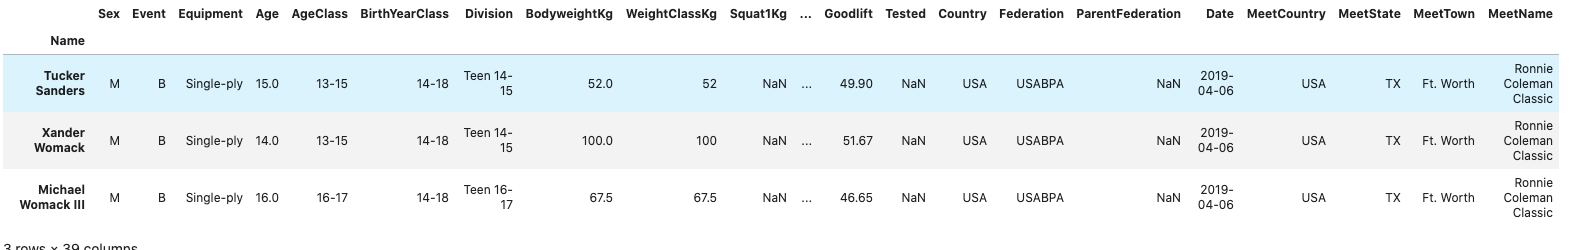
\includegraphics[width=\linewidth]{data_head.png}
\caption{データ全体}
\end{center}
\end{figure}

現状ではパワーリフティングの記録の回帰において必要のない指標も多く含まれているため、今回学習に使う指標は以下のみとする。

\begin{figure}[H]
\begin{center}
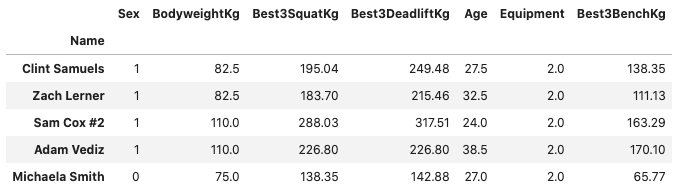
\includegraphics[width=\linewidth]{data_trimed.png}
\caption{使用するデータセット}
\end{center}
\end{figure}

それぞれの指標について簡単な説明を加えておく。一般的にパワーリフティングでは1回の試合において各競技3回まで試技を行う事が許されている。そのため、通常は試行回数を重ねるごとに記録は伸びる傾向にあるが、例えば2回目の試技では重量を持ち上げることに成功したが3回目の試技では失敗してしまった場合、3回目の試技欄には空白が入ることとなる。そのため、今回学習に用いるデータにおいてはそれぞれの試技において最高重量のみを抽出したものを使用している。また、パワーリフティングでは大会によって体にギア(図のEquipmentがそれにあたる)を着用する事が許されている場合があり、ギアを装着した場合は挙上重量が増加する傾向にある。また、それぞれの指標に対して、相関係数は下図のようになっている。

\begin{figure}[H]
\begin{center}
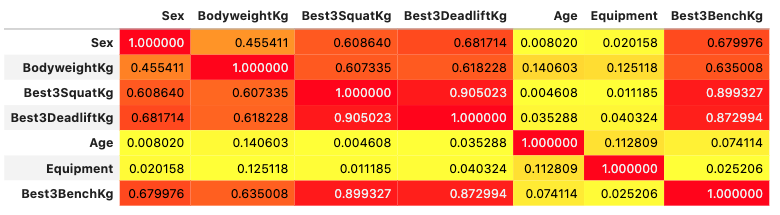
\includegraphics[width=\linewidth]{corr.png}
\caption{相関係数}
\end{center}
\end{figure}

相関係数数値は以下のような数式で表され、数値が1に近いほど相関があることを示している。

\begin{center}
\begin{math}
r_{xy} = \frac{\displaystyle \sum_{i = 1}^n (x_i - \overline{x})
(y_i - \overline{y})}{\sqrt{\displaystyle \sum_{i = 1}^n 
(x_i - \overline{x})^2}\sqrt{\displaystyle \sum_{i = 1}^n 
(y_i - \overline{y})^2}}
\end{math}
\end{center}

上記の表から、各競技(ベンチプレス・スクワット・デッドリフト)の重量はそれぞれ強い相関があることを示しており、年齢やギアと重量には相関が少ない事が伺える。

\section{評価指標}

回帰分析とは、説明変数\begin{math}X\end{math}に対し目的変数\begin{math}Y\end{math}が得られる分析の事である。したがって、正解値\begin{math}T\end{math}を目的変数\begin{math}Y\end{math}がどの程度正確に予測できいるかを調べる必要がある。今回の研究では、学習モデルの評価には決定係数(\begin{math}R^2\end{math})と平均絶対誤差(MAE)の2つの指標を用いることとする。

\subsection{決定係数}

決定係数は予測値\begin{math}Y\end{math}と正解値\begin{math}T\end{math}の相関を表す。一般的に決定係数は\begin{math}R^2\end{math}で示され、以下の数式で表される。

\begin{center}
\begin{math}R^2=1-\frac{\sum_{i=1}^{n}(T_i-\hat{Y_i})^2}{\sum_{i=1}^{n}(T_i-\bar{Y_i})^2}\end{math}
\end{center}

\begin{math}R^2\end{math}は予測値\begin{math}Y\end{math}と正解値\begin{math}T\end{math}が完全に一致する場合に1となり、1に近いほど精度の高い予測が行えていることを表す。


\subsection{平均絶対誤差}

平均絶対誤差(MAE)とは代表的な誤差関数の一つであり、以下のような数式で表される。

\begin{center}
\begin{math}
MAE = \frac{\sum_{i=1}^{n}|T_i-\hat{Y_i}|}{n} 
\end{math}
\end{center}

平均絶対誤差は尤度関数と密接に結びついている。他に尤度関数と密接に関係する指標として二乗平均平方根誤差(RMSE)が挙げられるが、平均絶対誤差は二乗平均平方根誤差に比べて外れ値の影響を受けにくいという特徴がある。パワーリフティングは、一般的にはベンチプレス・スクワット・デッドリフトの3種目の重量の合計値を競うものであるが、パワーリフティングの一種に他にもシングルベンチプレスという競技が存在し、こちらはベンチプレスの重量のみで勝敗を競うものである。こちらの競技の参加者は一般にスクワットやデッドリフトの重量に対してベンチプレスの重量が大きくなりやすく、今回のデータセットには多くの外れ値が含まれているという観点から、本研究では平均絶対誤差を評価精度として用いることとする。


\section{学習手法}
\subsection{多層パーセプトロン}

入力・出力以外にニューロン(隠れ層)が繋がったモデルを多層パーセプトロンと呼び、この手法を用いることで線形分離不可能なデータも扱う事ができる事は先述の通りである。

\subsection{活性化関数}

\subsubsection{Sigmoid関数}

\subsubsection{Tanh関数}

\subsection{最適化アルゴリズム}

\subsubsection{勾配降下法}

\subsubsection{Adam}

\section{Conclusion}
``I always thought something was fundamentally wrong with the universe'' \citep{adams1995hitchhiker}

\bibliographystyle{plain}
\bibliography{references}
\end{document}
